
In questo capitolo viene presentata la metodologia di validazione empirica adottata per misurare l'efficacia della metodologia proposta. L'obiettivo è quantificare il guadagno prestazionale offerto dal Fine-Tuning e dall'integrazione RAG rispetto a modelli base e a modelli generalisti allo stato dell'arte (SOTA).

\section{Configurazione dell'Esperimento}
\label{sec:exp_setup}

Per isolare il contributo delle singole componenti (Modello, Fine-Tuning, RAG), è stato disegnato un piano di test combinatorio che mette a confronto diverse configurazioni architetturali su un dataset di valutazione standardizzato.

\subsection{Modelli Oggetto di Studio}
Il benchmark coinvolge tre categorie di modelli, selezionati per rappresentare diversi paradigmi di approccio:

\begin{enumerate}
    \item \textbf{Non-Finetuned:}
    Sono state testate le versioni base dei modelli \texttt{Qwen3-32B} e \texttt{QwQ-32B}. Questi modelli possiedono solo la conoscenza acquisita durante il pre-training e servono come linea di base per valutare quanto il modello "grezzo" riesca a condurre analisi di vulnerabilità sul dominio specifico.
    
    \item \textbf{Modelli Specialized (Fine-Tuned):}
    Le versioni \texttt{Qwen3-32B-FT} e \texttt{QwQ-32B-FT}, risultanti dal processo di addestramento descritto nel Capitolo 3. Il confronto tra questi e le baseline permette di misurare il valore aggiunto specifico del Fine-Tuning.
    
    \item \textbf{Modello SOTA Generalista:}
    È stato incluso nel test \texttt{DeepSeek-V3} (tramite API), un modello di scala massiva (>600B parametri MoE). Questo rappresenta il "gold standard" attuale dei modelli open-weights e serve a rispondere alla domanda di ricerca sulla validità dei modelli piccoli specializzati contro i modelli giganti generalisti.
\end{enumerate}

\subsection{Modalità di Inferenza}
Ogni modello è stato testato in due modalità operative distinte per valutare l'impatto della pipeline RAG:

\begin{itemize}
    \item \textbf{Modalità No-RAG (Direct Prompting):} Il modello riceve in input solo il codice del contratto e l'istruzione di audit. Questa modalità misura la "conoscenza parametrica" intrinseca del modello.
    \item \textbf{Modalità With-RAG:} Il modello riceve il prompt ingegnerizzato contenente la \textit{Dynamic Checklist} e gli snippet \textit{Few-Shot} recuperati dal sistema RAG. Questa modalità misura la capacità del modello di sfruttare il contesto esterno ("conoscenza non parametrica").
\end{itemize}

\section{Dataset di Validazione (Test Set)}
Per garantire l'integrità dei risultati, la valutazione è stata condotta su un \textbf{Test Set isolato}, composto da smart contract mai visti dai modelli durante la fase di training.
Il corpus di test comprende un totale di \textbf{45 smart contract}, bilanciati per verificare sia la capacità di rilevamento che la robustezza ai falsi positivi:

\begin{itemize}
    \item \textbf{40 Contratti Vulnerabili:} Distribuiti equamente tra le 8 classi di vulnerabilità analizzate (5 esempi per classe). Ogni contratto contiene un'unica vulnerabilità nota e verificata, che funge da \textit{Ground Truth}.
    \item \textbf{5 Contratti Sicuri (Safe):} Contratti privi di vulnerabilità, inseriti per testare la tendenza del modello ad "allucinare" problemi inesistenti (False Positive Rate).
\end{itemize}

\section{Metriche di Valutazione}
\label{sec:metrics}

La valutazione delle performance si basa sulla matrice di confusione classica, adattata al dominio dell'audit di sicurezza. Per ogni contratto analizzato, l'output del modello viene classificato come:

\begin{itemize}
    \item \textbf{True Positive (TP):} Il modello identifica correttamente la vulnerabilità specifica presente nel contratto.
    \item \textbf{False Negative (FN):} Il modello dichiara il contratto sicuro o identifica una vulnerabilità diversa da quella realmente presente (mancato rilevamento).
    \item \textbf{False Positive (FP):} Il modello segnala una vulnerabilità in un contratto sicuro, oppure segnala una vulnerabilità aggiuntiva inesistente in un contratto vulnerabile (falso allarme).
    \item \textbf{True Negative (TN):} Il modello classifica correttamente un contratto sicuro come privo di vulnerabilità.
\end{itemize}

A partire da questi valori, sono state calcolate le seguenti metriche derivate:

\begin{equation}
    \text{Accuracy} = \frac{TP + TN}{TP + TN + FP + FN}
\end{equation}
Misura la percentuale complessiva di predizioni corrette. Tuttavia, in contesti sbilanciati o critici come la sicurezza, l'accuratezza da sola può essere fuorviante.

\begin{equation}
    \text{Precision} = \frac{TP}{TP + FP}
\end{equation}
Indica l'affidabilità delle segnalazioni: quando il modello dice "c'è un bug", quante volte ha ragione? Una bassa precisione implica molti falsi allarmi, che causano "alert fatigue" negli auditor umani.

\begin{equation}
    \text{Recall (Sensitivity)} = \frac{TP}{TP + FN}
\end{equation}
Indica la capacità di copertura: quanti dei bug esistenti è riuscito a trovare? In ambito cybersecurity, questa è spesso la metrica più critica, poiché un FN (bug mancato) può portare a un exploit.

\begin{equation}
    \text{F1-Score} = 2 \cdot \frac{\text{Precision} \cdot \text{Recall}}{\text{Precision} + \text{Recall}}
\end{equation}
Rappresenta la media armonica tra Precision e Recall, fornendo una misura sintetica dell'equilibrio del modello.

\section{Pipeline di Valutazione Automatizzata}
\label{sec:eval_pipeline}

Data la necessità di valutare molteplici configurazioni su un dataset di 45 contratti, l'analisi manuale dei risultati sarebbe risultata inefficiente e soggetta a errore umano. È stata pertanto sviluppata una \textbf{Pipeline di Testing Automatizzata} in Python, in grado di gestire l'intero ciclo di vita dell'esperimento, dall'inferenza al calcolo delle metriche finali.

La Figura \ref{fig:eval_pipeline} illustra l'architettura del sistema di valutazione.

\subsection{Parsing Strutturale}
Il funzionamento della pipeline si basa sulla capacità dei modelli (particolarmente quelli Fine-Tuned) di generare output strutturati delimitate dai tag \texttt{<final>}.
\begin{enumerate}
    \item \textbf{Estrazione:} Il modulo parser analizza la risposta grezza tramite espressioni regolari (Regex) per isolare il contenuto del blocco \texttt{<final>}.
    \item \textbf{Validazione Sintattica:} Se il parser non trova i tag di chiusura o rileva un formato JSON corrotto, la risposta viene scartata e il prompt viene reinviato al modello, fino a un massimo di 3 tentativi. Questo garantisce che le metriche riflettano la capacità di reasoning e non vengano penalizzate da errori banali di formattazione.
\end{enumerate}

\subsection{Classificazione (TP/FP/FN/TN)}
Una volta estratto il verdetto (es. "Vulnerabilità rilevata: Rekeying"), questo viene confrontato con la \textit{Ground Truth} (l'etichetta reale del contratto nel dataset di test):
\begin{itemize}
    \item Se il verdetto coincide con l'etichetta $\rightarrow$ \textbf{True Positive (TP)}.
    \item Se il modello segnala "Sicuro" ma il contratto è vulnerabile $\rightarrow$ \textbf{False Negative (FN)}.
    \item Se il modello segnala una vulnerabilità diversa da quella reale o segnala un contratto sicuro come infetto $\rightarrow$ \textbf{False Positive (FP)}.
    \item Se il modello segnala "Sicuro" e il contratto è effettivamente sicuro $\rightarrow$ \textbf{True Negative (TN)}.
\end{itemize}
I risultati vengono aggregati in un registro persistente, che alimenta il modulo finale per il calcolo delle metriche di performance (Precision, Recall, F1-Score, Accuracy).

% --- DIAGRAMMA PIPELINE DI TEST ---
\begin{figure}[!h]
    \centering
    \begin{tikzpicture}[
        node distance=2.2cm,
        auto,
        block/.style={
            rectangle, 
            draw, 
            fill=blue!10, 
            text width=2.5cm, 
            text centered, 
            rounded corners, 
            minimum height=1.2cm,
            font=\small
        },
        decision/.style={
            diamond, 
            draw, 
            fill=yellow!10, 
            text width=1.8cm, 
            text centered, 
            inner sep=0pt,
            font=\footnotesize
        },
        cloud/.style={
            draw, 
            ellipse, 
            fill=green!10, 
            minimum height=0.8cm,
            text width=2cm, 
            text centered,
            font=\footnotesize
        },
        line/.style={draw, -latex', thick},
        retry/.style={draw, -latex', thick, red, dashed}
    ]

    % Nodes
    \node [cloud] (dataset) {Test Set (45 Contratti)};
    \node [block, below of=dataset] (inference) {Model Inference (LLM)};
    \node [block, below of=inference] (parser) {Output Parser (<final> tag)};
    
    % Decision Node
    \node [decision, below of=parser, node distance=2.5cm] (check) {Formato Valido?};
    
    % Branch Yes
    \node [block, below of=check, node distance=2.5cm] (comparator) {Confronto con Ground Truth};
    
    % Branch No (Retry) - posizionato a destra
    \node [decision, right of=check, node distance=4cm] (limit) {Max Retries?};
    
    % Classification Categories
    \node [block, below of=comparator] (classify) {Classificazione (TP, FP, FN, TN)};
    \node [block, below of=classify] (metrics) {Calcolo Metriche};

    % Edges
    \path [line] (dataset) -- (inference);
    \path [line] (inference) -- (parser);
    \path [line] (parser) -- (check);
    
    % Logic Yes
    \path [line] (check) -- node [near start, right] {Sì} (comparator);
    
    % Logic No -> Retry Loop
    \path [line] (check) -- node [near start, above] {No} (limit);
    \path [retry] (limit) |- node [ right] {Retry} (inference);
    \path [line] (limit) |- node [near start, right] {Sì (Fail)} (classify); % Se supera i tentativi fallisce (es. conta come FN o errore)
    
    % Ground Truth input
    \node [cloud, left of=comparator, node distance=3.5cm] (truth) {Ground Truth Labels};
    \path [line, dashed] (truth) -- (comparator);
    
    % Final Flow
    \path [line] (comparator) -- (classify);
    \path [line] (classify) -- (metrics);

    \end{tikzpicture}
    \caption{Diagramma della Pipeline di Valutazione.}
    \label{fig:eval_pipeline}
\end{figure}

\newpage
\section{Analisi dell'Impatto del Fine-Tuning}
\label{sec:impact_finetuning}

Il primo livello di analisi mira a quantificare il guadagno prestazionale ottenuto attraverso il processo di Fine-Tuning (FT), isolandolo dall'apporto del RAG. Il confronto viene effettuato tra i modelli \textit{Base} e le rispettive versioni \textit{Fine-Tuned}, mantenendo il prompt statico e valutando la capacità intrinseca del modello di adattarsi al dominio PyTeal.

\subsection{Valutazione Quantitativa: Il Salto Prestazionale}
Come evidenziato nella letteratura di riferimento, i modelli non \textit{Finetuned} faticano a interpretare linguaggi a basso livello come TEAL o PyTeal, dove la semantica è oscurata da una logica stack-based meno espressiva rispetto a Solidity o Rust.
I risultati sperimentali, riassunti nelle Figure \ref{fig:ft_impact_metrics_qwen} e \ref{fig:ft_impact_metrics_qwq}, confermano drasticamente questa ipotesi.


% --- GRAFICO A BARRE ---
\begin{figure}[h]
    \centering
    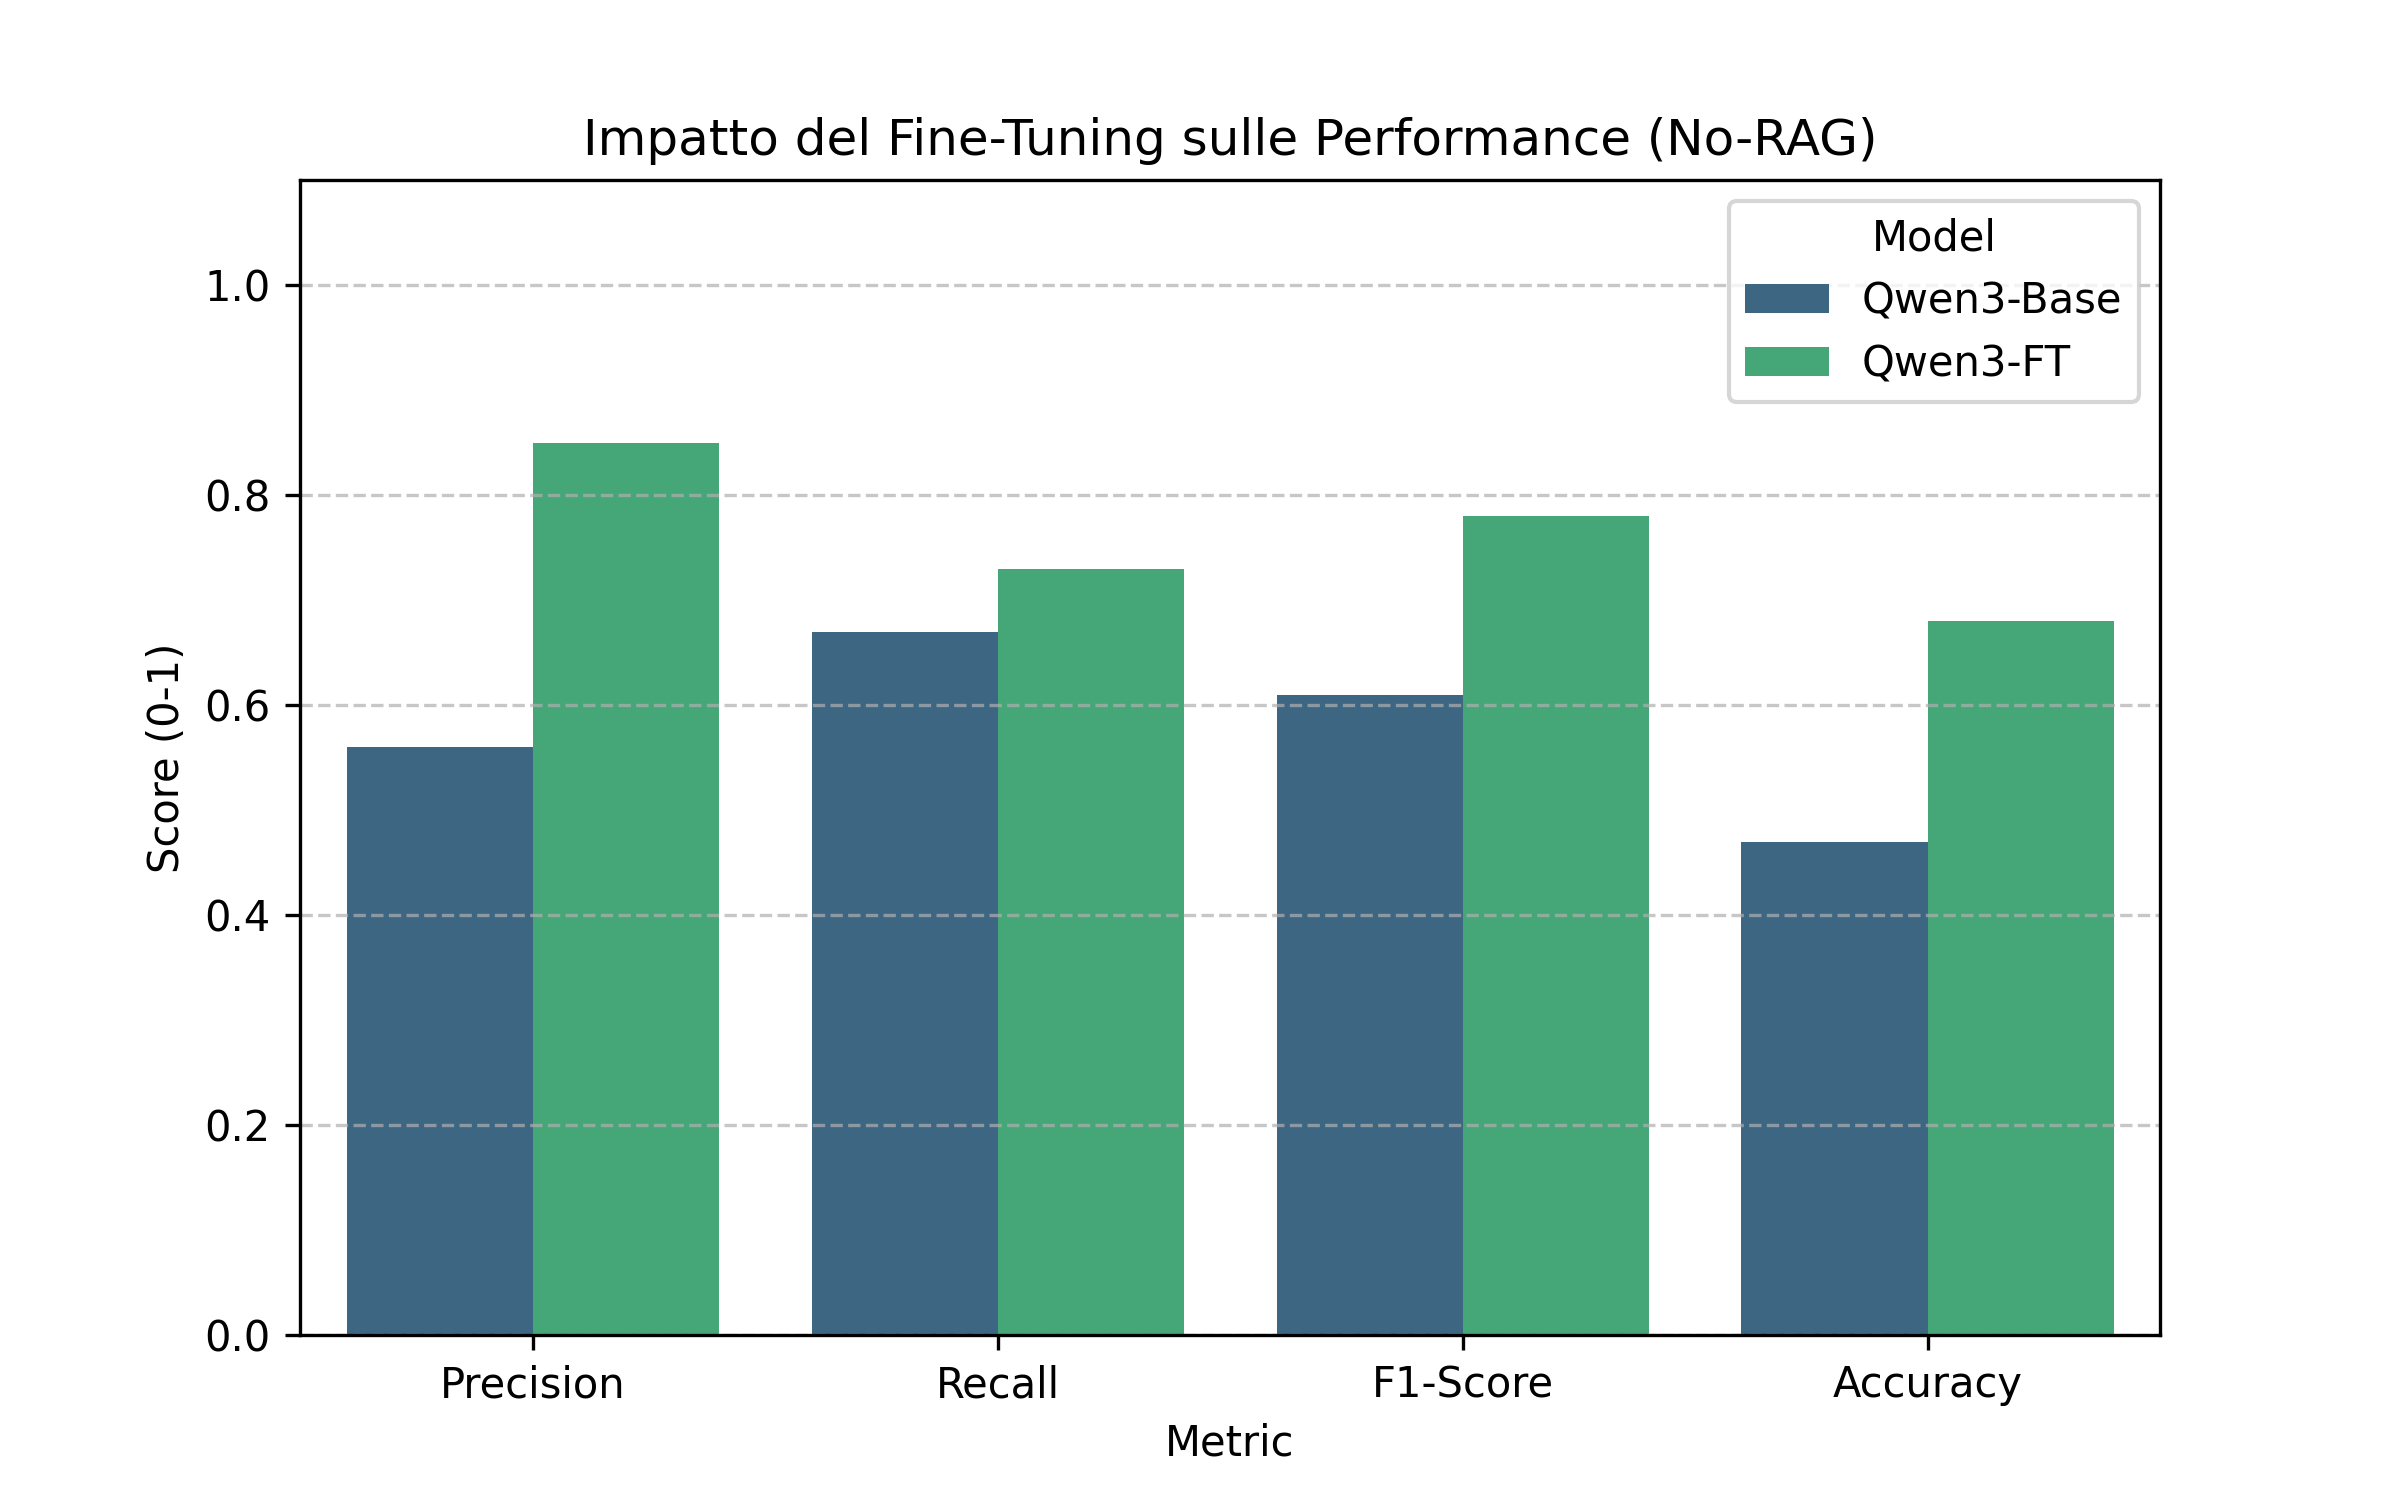
\includegraphics[width=0.9\textwidth]{images/ft_impact_chart_Qwen3.png}
    \caption{Impatto del Fine-Tuning (Qwen3) sulle metriche di performance (Accuracy, Precision, Recall, F1).}
    \label{fig:ft_impact_metrics_qwen}
\end{figure}

\begin{figure}[h]
    \centering
    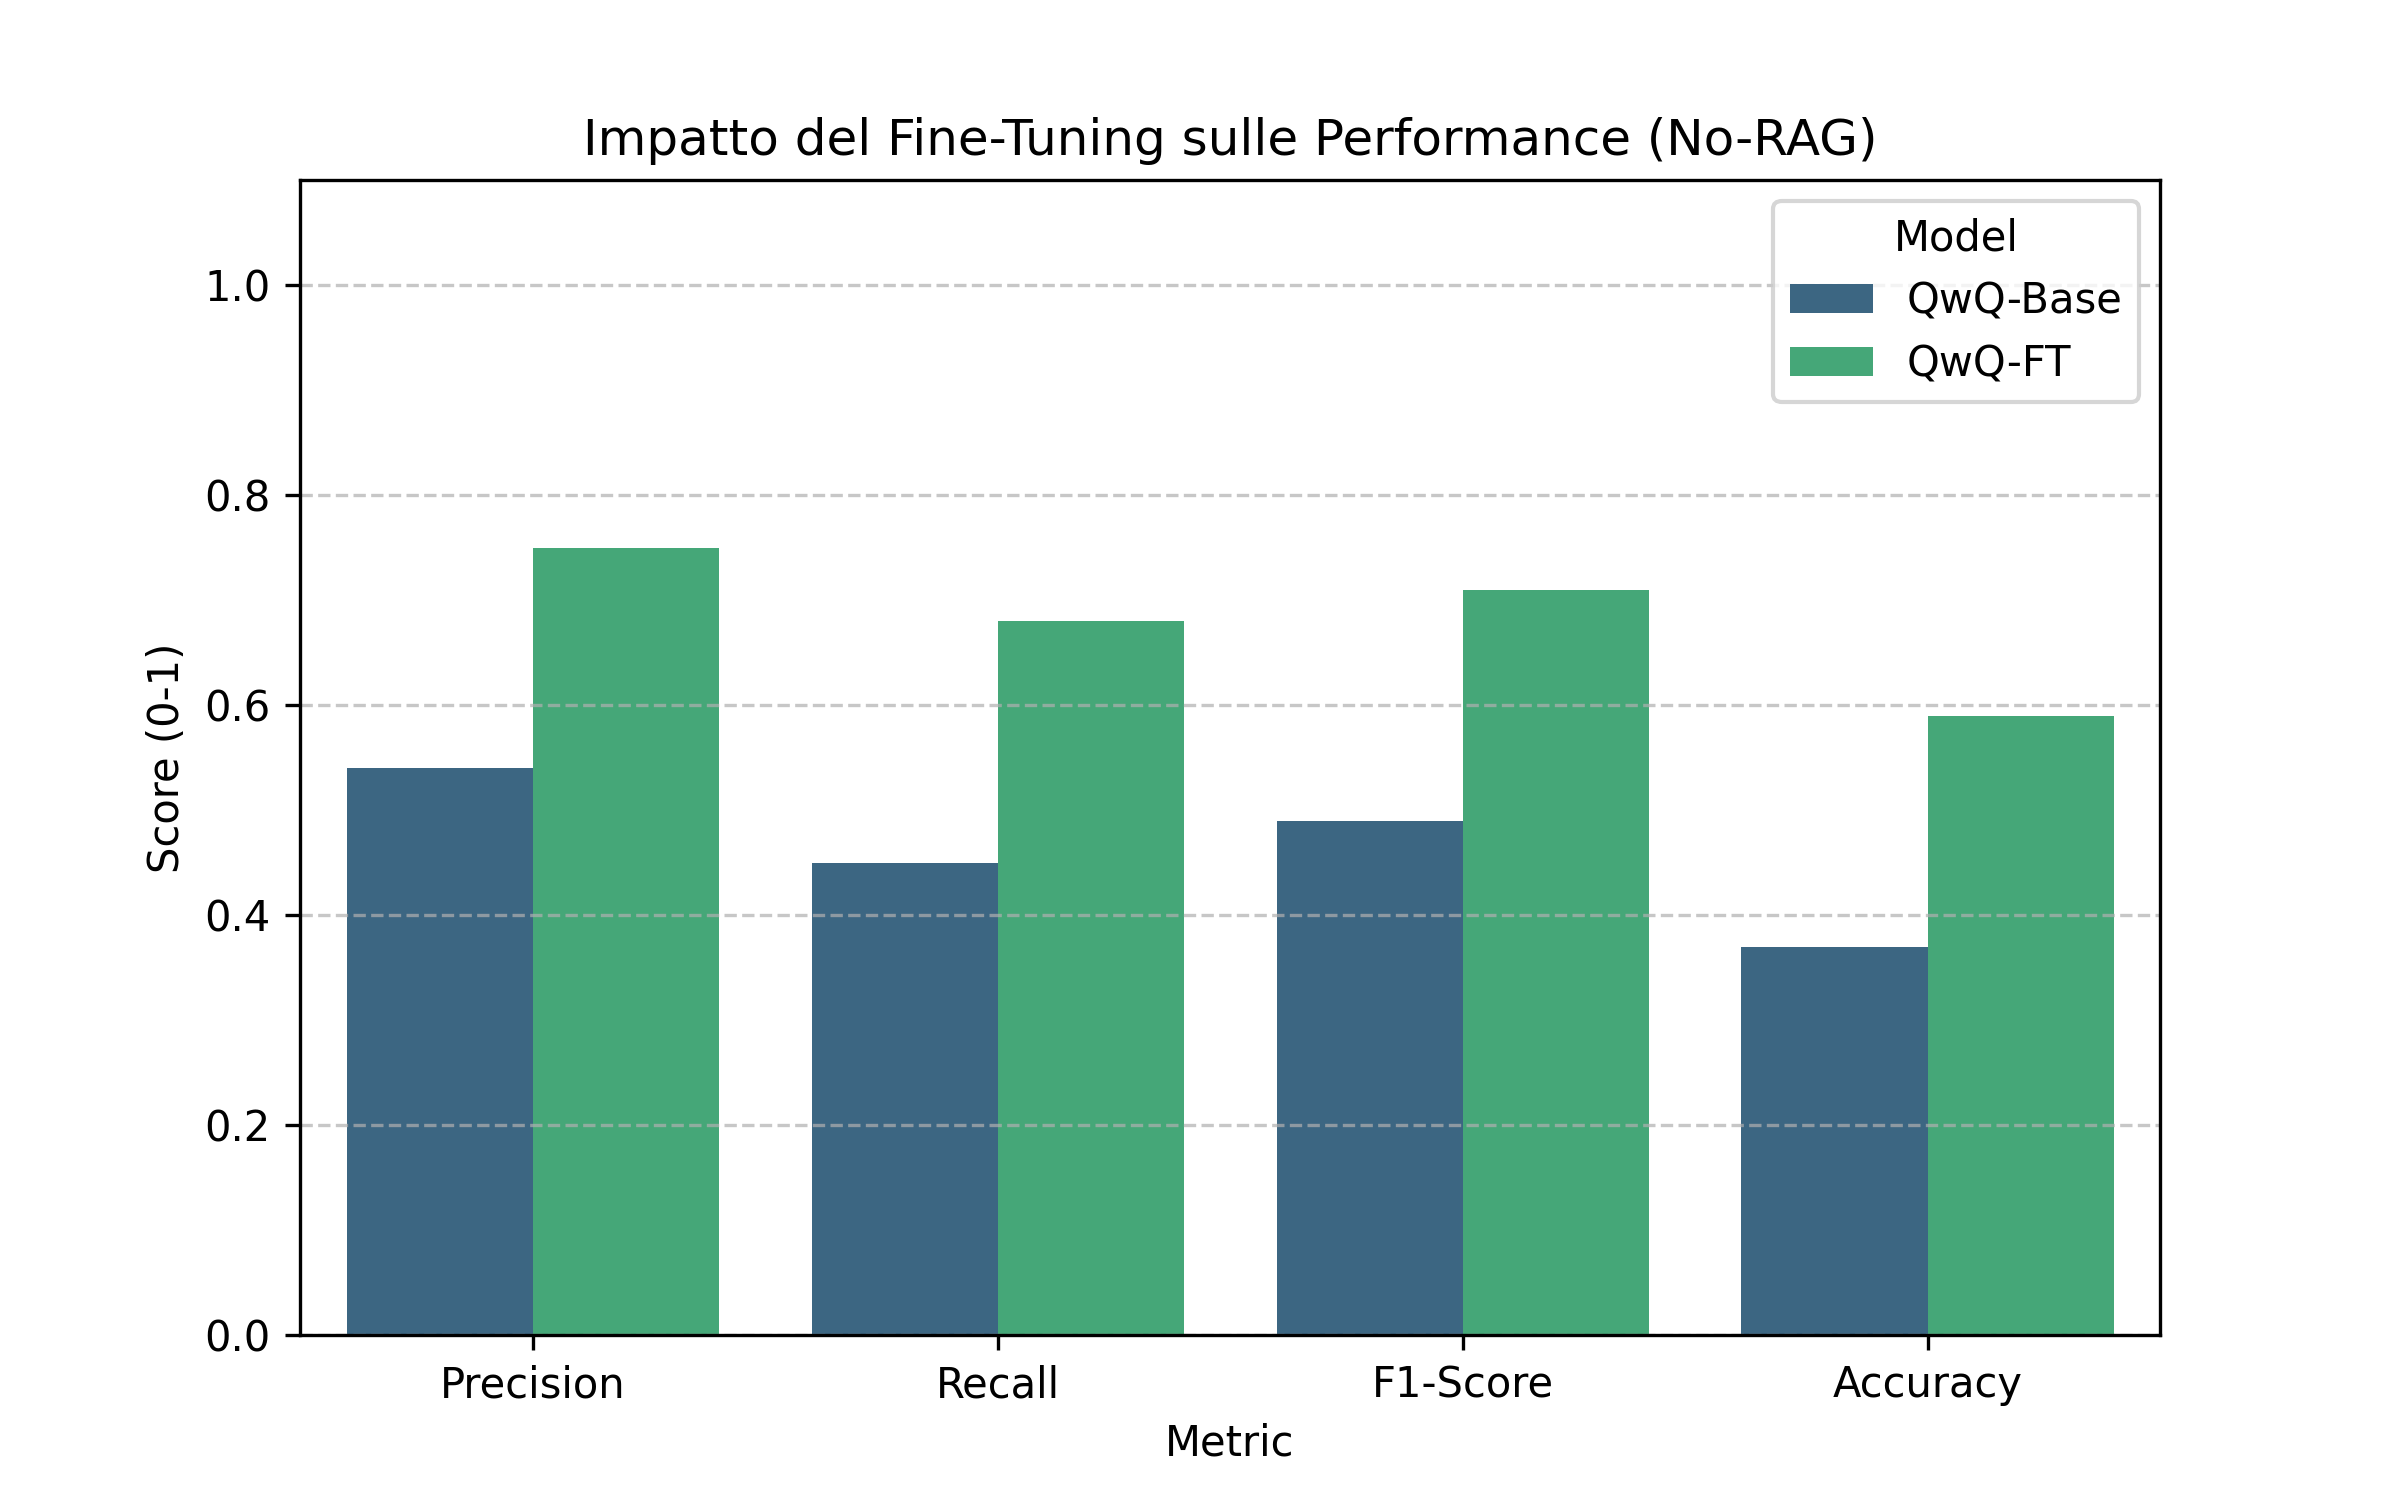
\includegraphics[width=0.9\textwidth]{images/ft_impact_chart_QwQ.png}
    \caption{Impatto del Fine-Tuning (QwQ) sulle metriche di performance (Accuracy, Precision, Recall, F1).}
    \label{fig:ft_impact_metrics_qwq}
\end{figure}

\newpage

Dall'analisi del grafico emergono trend distinti:
\begin{itemize}
    \item \textbf{Precision (Riduzione del Rumore):} È la metrica che ha beneficiato della trasformazione più radicale, smentendo l'ipotesi che il Fine-Tuning introduca overfitting. Al contrario, i dati mostrano che il modello Base soffriva di un elevato tasso di \textit{False Positives} (21 FP per Qwen3). Il modello FT ha imparato a discriminare i falsi allarmi, \textbf{abbattendo i FP a 5} e innalzando la Precision all'85\%.
    
    \item \textbf{Recall (Recupero della Conoscenza):} Per i modelli orientati al ragionamento (come QwQ), il Fine-Tuning è stato determinante per colmare il gap di conoscenza sintattica. Mentre il modello Base falliva nel riconoscere pattern specifici dell'AVM (con un alto tasso di FN), il processo di training ha permesso di "interiorizzare" le firme delle vulnerabilità, portando la Recall da un insufficiente 0.45 a un competitivo 0.675.
    
    \item \textbf{F1-Score e Affidabilità:} L'incremento dell'Accuracy non è solo numerico, ma qualitativo. Mentre l'accuratezza del modello Base era compromessa dall'incapacità di bilanciare sensibilità e specificità, il modello FT raggiunge un F1-Score di 0.78 (Qwen3), dimostrando di aver acquisito una comprensione operativa "utile": segnala le vulnerabilità quando ci sono e tace quando il codice è sicuro.
\end{itemize}

\begin{table}[h]
    \centering
    \caption{Dettaglio della Matrice di Confusione per i modelli testati (Test Set: 45 Contratti).}
    \label{tab:confusion_matrix_raw}
    \resizebox{\textwidth}{!}{%
    \begin{tabular}{l|cccc|c}
    \toprule
    \textbf{Modello} & \textbf{True Positive (TP)} & \textbf{True Negative (TN)} & \textbf{False Positive (FP)} & \textbf{False Negative (FN)} & \textbf{Totale} \\ \midrule
    Qwen3-32B (Base) & 27 & 4 & 21 & 13 & 65* \\
    \textbf{Qwen3-32B (FT)} & \textbf{29} & \textbf{5} & \textbf{5} & \textbf{11} & 50 \\ \midrule
    QwQ-32B (Base) & 18 & 4 & 15 & 22 & 59* \\
    \textbf{QwQ-32B (FT)} & \textbf{27} & \textbf{5} & \textbf{9} & \textbf{13} & 54 \\ \midrule
    
    \end{tabular}%
    }
    \vspace{0.2cm}
    \small
    \textit{*Nota: Per i modelli Base, la somma totale supera di molto 45 in quanto il modello tende a segnalare vulnerabilità multiple o errate (FP multipli) sullo stesso contratto.}
\end{table}

\subsection{Case Study Qualitativo}
\label{sec:case_study_rekey}

Per comprendere appieno il valore aggiunto del Fine-Tuning, è utile analizzare come i due modelli affrontano una vulnerabilità complessa basata su un'omissione: l'\textit{Unchecked Rekey To}.
In questo scenario, viene sottoposto ai modelli uno Smart Contract \textit{Stateless} (LogicSig) che approva un gruppo di due transazioni:
\begin{enumerate}
    \item \texttt{Gtxn[0]}: Una transazione di pagamento (Payment).
    \item \texttt{Gtxn[1]}: Un trasferimento di asset (AssetTransfer).
\end{enumerate}
Il codice è vulnerabile perché, mentre la seconda transazione controlla il campo \texttt{rekey\_to}, la prima (il pagamento) ne è priva, permettendo a un attaccante di prendere il controllo dell'account.

\subsubsection{Confronto delle Risposte}
Le Figure \ref{fig:resp_base} e \ref{fig:resp_ft} mostrano le risposte grezze generate rispettivamente dal modello Base e dal modello Fine-Tuned.
\newpage

\begin{figure}[h!]
    \centering
    \begin{tcolorbox}[colback=red!5!white, colframe=red!75!black, title=Risposta Modello Base (Qwen3-32B)]
    \small
    \textbf{<think>} 
    \[...\] Looking at the payment\_txn\_check for Gtxn[0], they check the type is Payment, amount is under 1M and close\_remainder\_to is zero. That seems good. \[...\]
    Now the asset\_transfer\_check for Gtxn[1]. They check rekey\_to is zero. \[...\]
    So all the relevant checks are present. No missing checks that would lead to the listed vulnerabilities. \\
    \textbf{</think>}
    
    \textbf{<final>} \\
    \textbf{Vulnerability: Not Vulnerable} \\
    Explanation: All relevant security checks are explicitly implemented for transaction fees, close\_remainder\_to, \textbf{rekey\_to}, asset\_close\_to, and receiver addresses.
    \textbf{</final>}
    \end{tcolorbox}
    \caption{Il Modello Base analizza i controlli presenti ma fallisce nel notare l'assenza del controllo sul Rekeying nella prima transazione, generando un Falso Negativo.}
    \label{fig:resp_base}
\end{figure}

\newpage

\begin{figure}[h!]
    \centering
    \begin{tcolorbox}[colback=green!5!white, colframe=green!75!black, title=Risposta Modello Fine-Tuned (Qwen3-32B-FT)]
    \small
    \textbf{<think>} \\
     \[...\]
    \textbf{Payment Transaction (Gtxn[0]):} \\
    - Type check: TxnType.Payment \\
    - Fee limit: `<= 1000` \checkmark\\
    - \textbf{Missing check: No validation of rekey\_to() field} 

    \[...\]
    
    \textbf{Asset Transfer Transaction (Gtxn[1]):} \\
    - Rekey to: == Global.zero\_address() \checkmark

     \[...\]
    
    The critical issue I notice is in the payment transaction validation. While the asset transfer transaction properly checks rekey\_to, the payment transaction completely omits this check. \\
    \textbf{</think>}
    
    \textbf{<final>} \\
    \textbf{Vulnerability: Unchecked Rekey To} \\
    Explanation: The payment transaction validation logic fails to check the rekey\_to field, allowing an attacker to include a rekey operation. \\
    \textbf{</final>}
    \end{tcolorbox}
    \caption{Il Modello FT adotta un approccio sistematico (checklist), identificando correttamente l'omissione nella prima transazione.}
    \label{fig:resp_ft}
\end{figure}
\newpage

\subsubsection{Discussione dell'Errore}
L'analisi comparativa evidenzia due comportamenti distinti:

\begin{itemize}
    \item \textbf{Generalizzazione Fallace del Modello Base:} Nel suo processo di pensiero (Figura \ref{fig:resp_base}), il modello nota che il \texttt{rekey\_to} è controllato nella seconda transazione. Tuttavia, nel verdetto finale, estende erroneamente questa proprietà all'intero contratto, dichiarando \textit{"All relevant security checks are explicitly implemented for... rekey\_to"}. Questa è una classica allucinazione da generalizzazione: il modello confonde la presenza \textit{locale} di un controllo con la sicurezza \textit{globale}.
    
    \item \textbf{Verifica Puntuale del Modello FT:} Il modello Fine-Tuned (Figura \ref{fig:resp_ft}) struttura il ragionamento separando nettamente le due transazioni (\texttt{Gtxn[0]} vs \texttt{Gtxn[1]}). Grazie all'addestramento su esempi di audit strutturati, il modello ha imparato a cercare attivamente l'assenza di vincoli, rilevando che la mancanza della riga \texttt{RekeyTo == ZeroAddress} nel blocco di pagamento costituisce una vulnerabilità critica.
\end{itemize}

Questo esempio dimostra come il Fine-Tuning non si limiti ad aggiungere conoscenza sintattica, ma modifichi il pattern di attenzione del modello, spostandolo da una lettura "riassuntiva" a una verifica "analitica" riga per riga.

\newpage

\subsection{Benchmark contro modelli SOTA}
\label{sec:benchmark_deepseek}

Per validare la reale efficacia del Fine-Tuning, i risultati ottenuti dai modelli specializzati (in particolare \texttt{Qwen3-32B-FT}) sono stati confrontati con \texttt{DeepSeek V3.2}, un modello allo Stato dell'Arte (SOTA) di dimensioni massicce, interrogato via API.

La Tabella mostra il confronto diretto tra il miglior modello Fine-Tuned e il modello SOTA.

\begin{table}[ht]
\centering
\resizebox{\textwidth}{!}{%
\begin{tabular}{l|cccc|cc}
\toprule
\textbf{Modello} & \textbf{Precision} & \textbf{Recall} & \textbf{F1-Score} & \textbf{Accuracy} & \textbf{FP} & \textbf{FN} \\ \midrule
\textbf{Qwen3-32B (FT)} & \textbf{0.85} & 0.725 & \textbf{0.784} & \textbf{0.680} & \textbf{5} & 11 \\ 
DeepSeek V3.2 (API) & 0.717 & \textbf{0.825} & 0.767 & 0.649 & 13 & \textbf{7} \\ \bottomrule
\end{tabular}%
}
\label{tab:rere}
\caption{Confronto tra il modello Fine-Tuned (Specialist) e DeepSeek V3.2 (Generalist).}
\end{table}

\begin{figure}[h]
    \centering
    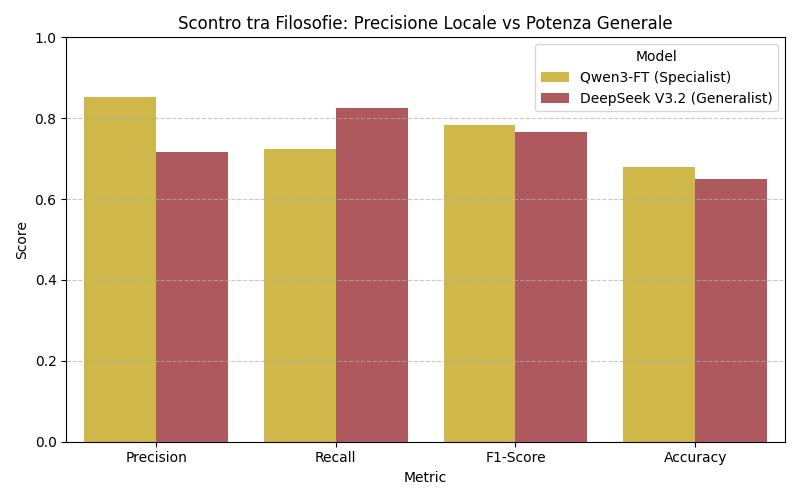
\includegraphics[width=0.9\textwidth]{images/ft_vs_deepseek.png}
    \caption{Confronto tra il modello Fine-Tuned (Specialist) e DeepSeek V3.2 (Generalist).}
    \label{fig:ft_vs_deepseek}
\end{figure}

Dall'analisi dei dati emerge una dinamica chiara che contrappone la "potenza bruta" alla "specializzazione":

\begin{itemize}
    \item \textbf{DeepSeek:} Grazie alla sua vasta conoscenza parametrica e capacità di ragionamento, DeepSeek ha ottenuto la \textbf{Recall più alta (0.825)}, identificando 33 vulnerabilità su 40 (solo 7 FN). Il modello riesce a trovare bug complessi che sfuggono al modello 32B, dimostrando che la capacità di ragionamento puro può compensare parzialmente la mancanza di training specifico.
    
    \item \textbf{Qwen3-FT:} Il modello Fine-Tuned, pur avendo una Recall inferiore (0.725), eccelle nella precisione. Con una \textbf{Precision dell'85\%} e solo \textbf{5 False Positives} (contro i 13 di DeepSeek), il modello specializzato si rivela molto più affidabile.
    
    \item \textbf{Accuracy e Affidabilità Globale:} Analizzando l'Accuracy, il modello FT supera il modello SOTA (\textbf{0.680 vs 0.649}). Questo dato, sebbene spesso meno informativo in dataset sbilanciati, qui conferma una tesi importante: DeepSeek "guadagna" Recall sparando nel mucchio (generando molti FP), mentre Qwen3-FT commette meno errori totali (somma di FP e FN).
    
    \item \textbf{F1-Score:} La sintesi finale premia l'equilibrio del modello specializzato (\textbf{0.784 vs 0.767}). Dimostra che un modello compatto (32B), se correttamente addestrato, può competere e superare un modello SOTA di ordine di grandezza superiore.
\end{itemize}

\section{Analisi Comparativa dell'Impatto del RAG}
\label{sec:rag_impact_analysis}

L'introduzione della pipeline RAG (Retrieval-Augmented Generation) rappresenta l'ultimo stadio di ottimizzazione del framework. In questa sezione analizziamo come l'iniezione di contesto dinamico influenzi le performance di tutte e cinque le configurazioni di modello testate, confrontando le metriche \textit{No-RAG} contro \textit{With-RAG}.

La Tabella \ref{tab:rag_comparison_full} riassume i delta prestazionali per tutte le metriche chiave.

\begin{table}[ht]
\centering
\resizebox{\textwidth}{!}{%
\begin{tabular}{l|cc|cc|cc}
\toprule
\textbf{Modello} & \multicolumn{2}{c|}{\textbf{Precision}} & \multicolumn{2}{c|}{\textbf{Recall}} & \multicolumn{2}{c}{\textbf{F1-Score}} \\ 
 & No-RAG & \textbf{With RAG} & No-RAG & \textbf{With RAG} & No-RAG & \textbf{With RAG} \\ \midrule
\textit{Base Models} & & & & & & \\
QwQ-32B & 0.57 & \textbf{0.83 (+0.26)} & 0.45 & \textbf{0.60 (+0.15)} & 0.51 & \textbf{0.70 (+0.19)} \\
Qwen3-32B & 0.56 & \textbf{0.90 (+0.34)} & 0.67 & 0.65 (-0.02) & 0.61 & \textbf{0.75 (+0.14)} \\ \midrule
\textit{Fine-Tuned Models} & & & & & & \\
\textbf{QwQ-32B (FT)} & 0.83 & \textbf{0.92 (+0.09)} & 0.72 & \textbf{0.87 (+0.15)} & 0.77 & \textbf{0.90 (+0.13)} \\
Qwen3-32B (FT) & 0.85 & \textbf{0.94 (+0.09)} & 0.72 & \textbf{0.82 (+0.10)} & 0.78 & \textbf{0.88 (+0.10)} \\ \midrule
\textit{SOTA} & & & & & & \\
DeepSeek V3.2 & 0.73 & \textbf{0.91 (+0.18)} & 0.82 & \textbf{0.97 (+0.15)} & 0.77 & \textbf{0.94 (+0.17)} \\ \bottomrule
\end{tabular}%
}
\caption{Impatto del RAG su Precision, Recall e F1-Score. I valori tra parentesi indicano il guadagno netto ($\Delta$) rispetto alla versione senza RAG.}
\label{tab:rag_comparison_full}
\end{table}

\newpage

\begin{figure}[h!]
    \centering
    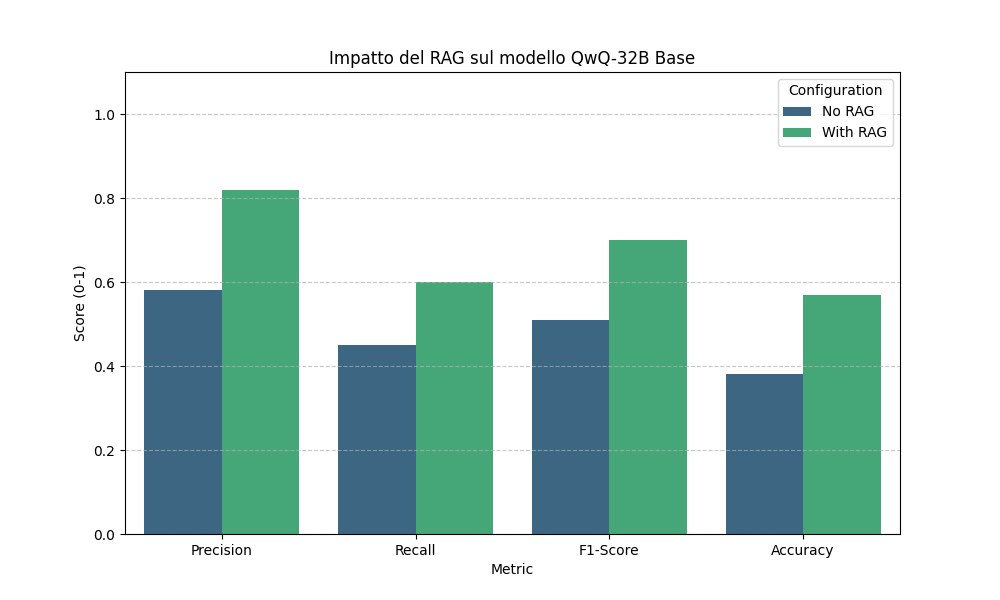
\includegraphics[width=\textwidth]{images/rag_impact_chart_qwq_base.png} 
    \caption{Confronto performance del modello QwQ-32B Base, con e senza RAG}
    \label{fig:rag_qwq_base}
\end{figure}

\begin{figure}[h!]
    \centering
    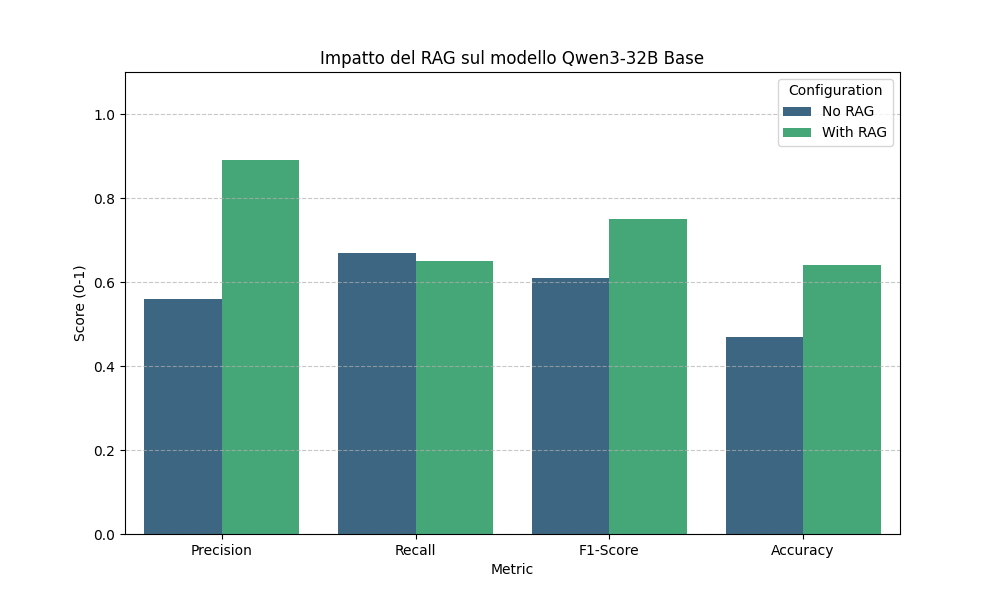
\includegraphics[width=\textwidth]{images/rag_impact_chart_qwen_base.png} 
    \caption{Confronto performance del modello Qwen3-32B Base, con e senza RAG}
    \label{fig:rag_qwen_base}
\end{figure}


\begin{figure}[h!]
    \centering
    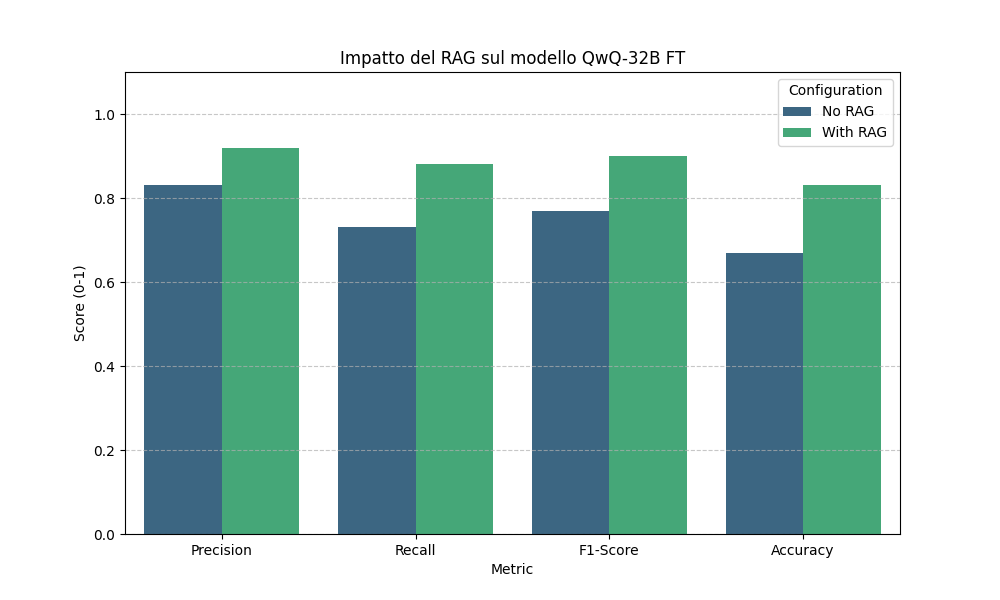
\includegraphics[width=\textwidth]{images/rag_impact_chart_qwq_ft.png} 
    \caption{Confronto performance del modello QwQ-32B FT, con e senza RAG}
    \label{fig:rag_qwq_ft}
\end{figure}

\begin{figure}[h!]
    \centering
    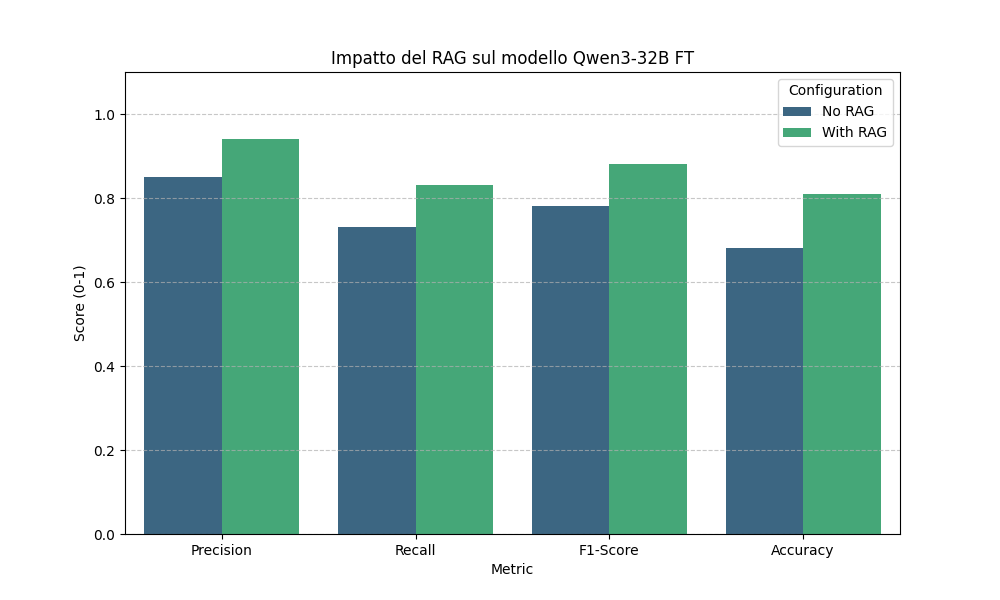
\includegraphics[width=\textwidth]{images/rag_impact_chart_qwen_ft.png} 
    \caption{Confronto performance del modello Qwen3-32B FT, con e senza RAG}
    \label{fig:rag_qwen_ft}
\end{figure}

\begin{figure}[h!]
    \centering
    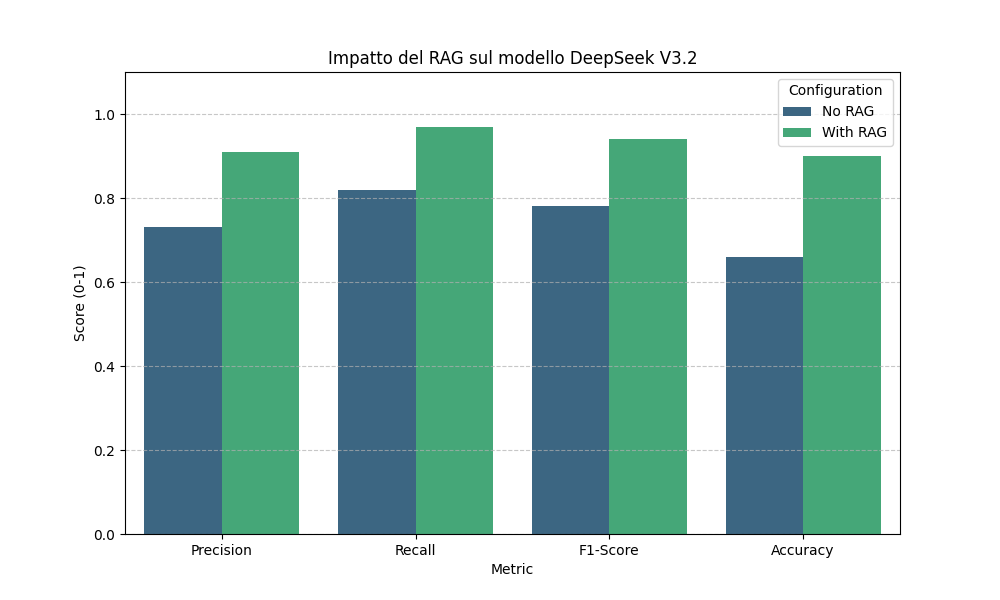
\includegraphics[width=\textwidth]{images/rag_impact_chart_deepseek.png} 
    \caption{Confronto performance del modello DeepSeek V3.2, con e senza RAG}
    \label{fig:rag_deepseek}
\end{figure}

\newpage

L'impatto del RAG si manifesta con dinamiche distinte in base alla maturità del modello sottostante.
Per i \textbf{Modelli Base} (QwQ/Qwen3), il retrieval agisce primariamente come "filtro di rumore": fornendo esempi reali, riduce drasticamente le allucinazioni (False Positives), portando la Precision dal 56\% all'89\% su Qwen3.
Nei \textbf{Modelli Fine-Tuned}, osserviamo la sinergia più efficace in termini di bilanciamento: il training pregresso garantisce la comprensione sintattica, mentre il RAG estende la memoria, permettendo al modello locale \texttt{QwQ-FT} di raggiungere un F1-Score di 0.90, rendendolo un'alternativa competitiva on-premise.
Infine, per il modello SOTA \textbf{DeepSeek V3.2}, il RAG colma le residue lacune di dominio: con una Recall del 97.5\% (un solo bug mancato su 40), dimostra che anche i modelli massivi necessitano di contesto specifico per saturare le performance su linguaggi di nicchia come PyTeal.

\subsection{Trade-off Computazionale e Latenza}
L'integrazione del RAG comporta inevitabilmente un costo computazionale aggiuntivo. Rispetto all'inferenza diretta, la pipeline ibrida introduce due fattori di overhead:
\begin{enumerate}
    \item \textbf{Latenza di Retrieval:} Il tempo necessario per l'embedding della query e la ricerca vettoriale (Vector Search) aggiunge circa 200-500ms per transazione analizzata.
    \item \textbf{Consumo di Token:} L'iniezione degli snippet di contesto nel prompt aumenta la finestra di input media del 40-60\%, incrementando proporzionalmente i tempi di pre-fill e i costi di inferenza (nel caso di API a pagamento).
\end{enumerate}
Tuttavia, considerando il dominio di applicazione (sicurezza degli Smart Contract), questo trade-off è ampiamente giustificato. In uno scenario di audit, dove l'accuratezza (F1-Score) è critica per prevenire perdite finanziarie, un incremento della latenza nell'ordine dei secondi è trascurabile rispetto al valore aggiunto della riduzione dei Falsi Negativi.

\subsection{Sintesi dei Risultati}
L'analisi comparata dimostra che:
\begin{enumerate}
    \item \textbf{Il RAG è sempre additivo:} Nessun modello ha peggiorato significativamente le performance globali con l'aggiunta del contesto.
    \item \textbf{FT + RAG > Base + RAG:} Il Fine-Tuning è un prerequisito essenziale per massimizzare l'efficacia del retrieval. QwQ-FT con RAG (F1 0.90) supera nettamente QwQ Base con RAG (F1 0.70), provando che il contesto non può sostituire completamente l'addestramento.
    \item \textbf{Gap SOTA ridotto:} La nostra soluzione locale (QwQ-FT + RAG) raggiunge un F1 di 0.90, distaccandosi di soli 4 punti percentuali dalla soluzione SOTA via API (0.94), validando la fattibilità di audit di sicurezza avanzati eseguiti on-premise.
\end{enumerate}